\chapter{Computational advantage} \label{Computational advantage}

\section{Benchmarking quantum computers}
As increasingly capable quantum computers are built and deployed, it is important to develop benchmarks that track the performance of these systems. The main goals of these benchmarks are to identify the necessary technology for each specific application and to link the debate on quantum advantage, i.e. where a user can run a quantum program to and a solution faster, cheaper or more accurately than classical computing alone, to the specific hardware that can achieve such calculation. \\
Unlike classical computer systems, where instructions are executed directly by a CPU, the Quantum Processing Unit (QPU), which is the combination of the control electronics and quantum memory, is supported by a classical runtime system for converting the circuits into a form consumable by the QPU and then retrieving results for further processing. Performance on actual applications depends on the performance of the complete system and, as such, any performance metric must holistically consider all of the components. \\
The performance of a quantum computer is governed by three key factors \cite{Wack2021Oct}:
\begin{itemize}
    \item \textbf{Scale:} \\
    It determines the size of problem that can be encoded and solved. The technological parameter that defines the scale of a quantum computer is the number of qubits;
    
    \item \textbf{Quality:} \\
    It determines the size of a quantum circuit that can be faithfully executed. The technological parameter for the quality of a quantum computer is the quantum volume (QV);
    
    \item \textbf{Speed:} \\
    It is related to the number of primitive circuits that the quantum computing system can execute per unit of time. The technological parameter that defines the speed of a quantum computer is the circuit layer operations per second (CLOPS);
\end{itemize}

\subsection{Number of qubits}
The number of qubits determines the amount of information that can be encoded in a quantum computer for computation, which caps the size of solvable problems. In quantum simulation the number of qubits sets the size of the basis set that represents each electron wave function in a molecule and therefore the size of the molecules that can be simulated. Number of qubits can also be used as a resource to improve the other two metrics of quality and speed. For example, auxiliary qubits can often be used to reduce the depth of circuits and increase their fidelity. Extra qubits can also be used in multiprogramming of QPUs to increase their circuit processing speed. \\
For most quantum computing platforms increasing the number of qubits, i.e. the scalability, relies heavily on the available materials and fabrication technologies developed from the semiconducting industry (superconducting, semiconducting, ion traps and photonics qubit platforms). While all quantum hardware platforms have challenges in scaling, superconducting qubits are making fast progress to scale beyond 100 qubits. \\
\\
The performance metrics to choose depend on the level of complexity one wants to capture with them. A useful way of thinking about it is a benchmarking pyramid, as shown in Figure \ref{Benchmarking pyramid}.
\begin{figure}[ht]
  \centering
  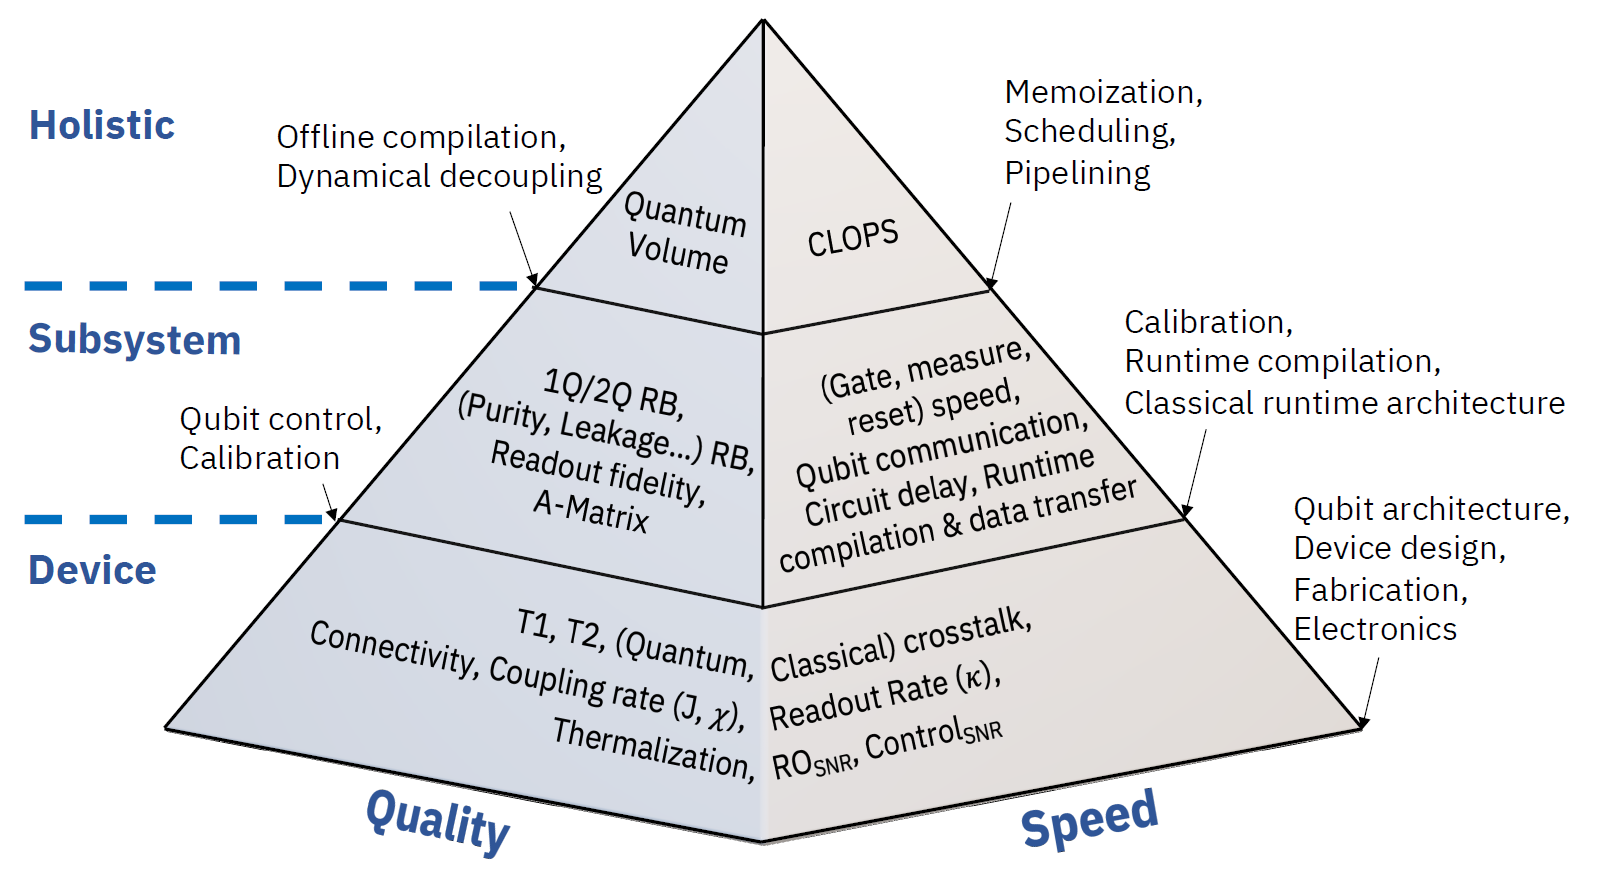
\includegraphics[width=0.8\textwidth]{figures/Benchmarking pyramid.png}
  \caption{Benchmarking pyramid. Higher-level benchmarks capture more complexity but less specificity \cite{Wack2021Oct}.} \label{Benchmarking pyramid}
\end{figure}

\subsection{Quantum volume}
Quantum volume (QV) indicates how faithfully a quantum circuit can be implemented in a quantum computing system. A QV layer is defined as one layer of permutation among qubits and one layer of pair-wise random SU(4) 2-qubit unitary gates. The QV is defined by the width or number of QV layers of the largest random square circuit (with width equal to the number of layers) that a quantum processor can successfully run. Note that, when a QV circuit is compiled to the native gate set of a particular QPU, the circuit depth of the compiled circuit will typically be much larger than the number of QV layers as the abstract permutations and SU(4) unitaries may be each decomposed into multiple native gates. \\
QV measurement starts with executing a square circuit of width $N$ and then compares the measurement results from the heavy output states (the states with probabilities higher than the median of probabilities of all output states) with the ideal results from simulation. The largest $N$-qubits square circuit that can run successfully to produce more than 2/3 of heavy outputs determines the quantum volume on a quantum computing system, given by $2N$. \\
QV is sensitive to coherence, gate fidelity and measurement fidelity, which are hardware properties of a quantum processor. It is also influenced by connectivity and compilers, which can make circuits efficient to minimize the effect of decoherence. \\
QV is a holistic metric because it cannot be improved by just improving one aspect of the system, but rather requires all parts of the system to be improved in a synergistic manner. It has been adopted widely by research and industry and has been reported for several ion trap and superconducting quantum computers.

\subsection{Circuit Layer Operations per Second Benchmark}
Circuit layer operations per second (CLOPS) is a measure correlated with how many QV circuits a QPU can execute per unit of time. \\
A. Wack et al. \cite{Wack2021Oct} formally defined as: the number of QV layers executed per second using a set of parameterized QV circuits, where each QV circuit has $D = log_2$ QV layers. Circuit execution time includes updating parameters to the circuit, submitting the job to the QPU, executing on the QPU and sending results back to be processed. CLOPS is then calculated as the total number of QV layers executed divided by the total execution time. \\
The CLOPS benchmark is designed to allow the system to leverage all of the quantum resources on a device to run a collection of circuits as fast as possible as well as to stress all parts of the execution pipeline. This includes data transfer of circuits and results, runtime compilation (lowering basis-gate level circuits to control electronics instructions), latencies in loading control electronics, initialization of control electronics, gate times, measurement times, reset time of qubits, delays between circuits, processing results and parameterized updates. The generation of random parameters from a seed constructed from the shots of the previous execution simulates the parameter updates in iterative quantum algorithms. \\
Including all of these parameters in the benchmark ensures that all aspects of the system are included to generate a meaningful comparison between systems. Physical qubit architectures may effect the repetition time, gate times, reset times and measurement times and can vary significantly across technologies. For example, the repetition rate and the gate rate of superconducting qubits can be orders of magnitude faster than the ones of ion trap qubits which significantly impacts the CLOPS. Similarly, software components such as runtime compilation, orchestration of the control electronics, etc. are all aspects that are necessary in current architectures to run already compiled programs for the QPU and have considerable impact on the overall performance. Finally the CLOPS is also impacted by how efficiently circuits can be delivered to the system for execution and results returned to the user-space application.

\subsection{Today's quantum computers}
Quantum computers already available come with a series of technological parameters useful to describe and improve them. \\
Here we take IBM quantum computers \cite{BibEntry2022Sep} as an example to show them. \\
The most fundamental technological parameters one can refer to are:
\begin{itemize}
    \item \textbf{Number of qubits, QV and CLOPS}: defined before;
    
    \item \textbf{Connectivity}: how the links between the single qubits in the processor are prepared, e.g. linear or full connectivity. It is also shown by a map of the processor;
    
    \item $T_1$: the longitudinal relaxation time of the higher energy $\ket{1}$ state into ground state $\ket{0}$, i.e. the classical state lifetime;
    
    \item $T_2$: the transverse relaxation time of superposition states such as $\frac{\ket{0} + \ket{1}}{\sqrt{2}}$, i.e. the dephasing time. \\
    $T_1$ and $T_2$ are generally referred to as 'decoherence time';
    
    \item \textbf{Frequency}: the qubits from IBM are superconducting qubits, thus interactions with these qubits are performed via microwave resonators. To address each different qubit separately each qubits resonator has a different frequency. This value is defined as the energy difference between the $\ket{0}$ and $\ket{1}$ states;
    
    \item \textbf{Readout assignment error}: the measure of how well the measurement performs, more formally, the probability of a measurement returning the wrong value;
    
    \item \textbf{Prob meas0 prep1}: the probability that a measurement returns $0$ immediately after preparing the $\ket{1}$ state. A combination of faulty preparation and faulty measurement. These are also often referred to as SPAM (state-preparation-and-measurement) errors;
    
    \item \textbf{Prob meas1 prep0}: likewise the previous one, but for the $\ket{0}$ state;
    
    \item \textbf{Readout length (ns)}: the time it takes to perform a measurement (in ns). This is one of the main limiting factors of current quantum hardware as these times are often considerably longer than the $T_2$, which makes intermediate measurements, i.e. measurements that are not at the end of a circuit, practically unfeasible;
    
    \item \textbf{ID error}: the measure of the error induced by having the qubit idle for a typical gate time. The measure used is the one returned by randomized benchmarking, which closely resembles the process fidelity;
    
    \item $\sqrt{X}$ \textbf{error}: the measure of error induced by applying the $\sqrt{X}$ gate. Average over all different qubits;
    
    \item \textbf{Single-qubit Pauli $X$ error}: likewise the previous one, but for the $X$ gate;
    
    \item \textbf{CNOT error}: the error of the only two-qubits gate natively implementable on the devices. Average over all possible CNOT gates;
    
    \item \textbf{Gate time (ns)}: the time it takes to perform a CNOT gate.
\end{itemize}
As of today IBM has released a 127-qubits processor called ibm\_washington, but, as we have described before, this fact does not tell the whole story, in fact this processor has a QV of 64 and CLOPS of 850, while a 27-qubits processor called ibmq\_montreal has a QV of 128 and CLOPS of 2000. Moreover, a 7-qubits processor called ibm\_perth, built with the same technology, has CLOPS of 2900, one of the highest already available. The highest value of QV, as of today, has been reached by the company Quantinuum with the System Model H1-2 which presents a QV of 4096. \\
A more precise analysis on the relations between different technological parameters, especially the number of qubits and CLOPS, can be made by breaking down the time to execute the benchmark into different areas \cite{Wack2021Oct}. \\
\\
These and many other companies frequently present roadmaps for the technology advancements in the quantum computers they build. Some focus more on scale up rapidly the number of qubits to run complex calculations, some focus on achieving a high quality before the progress in scale takes place, i.e. build logical qubits by implementation of error-correction codes and high QV devices. \\
Below we show the roadmaps from IBM and Google and a general one representing different companies with different technologies. This is a useful instrument to carry out an analysis and a forecast of the applications that will be available in the future years.
\begin{figure}[ht]
  \centering
  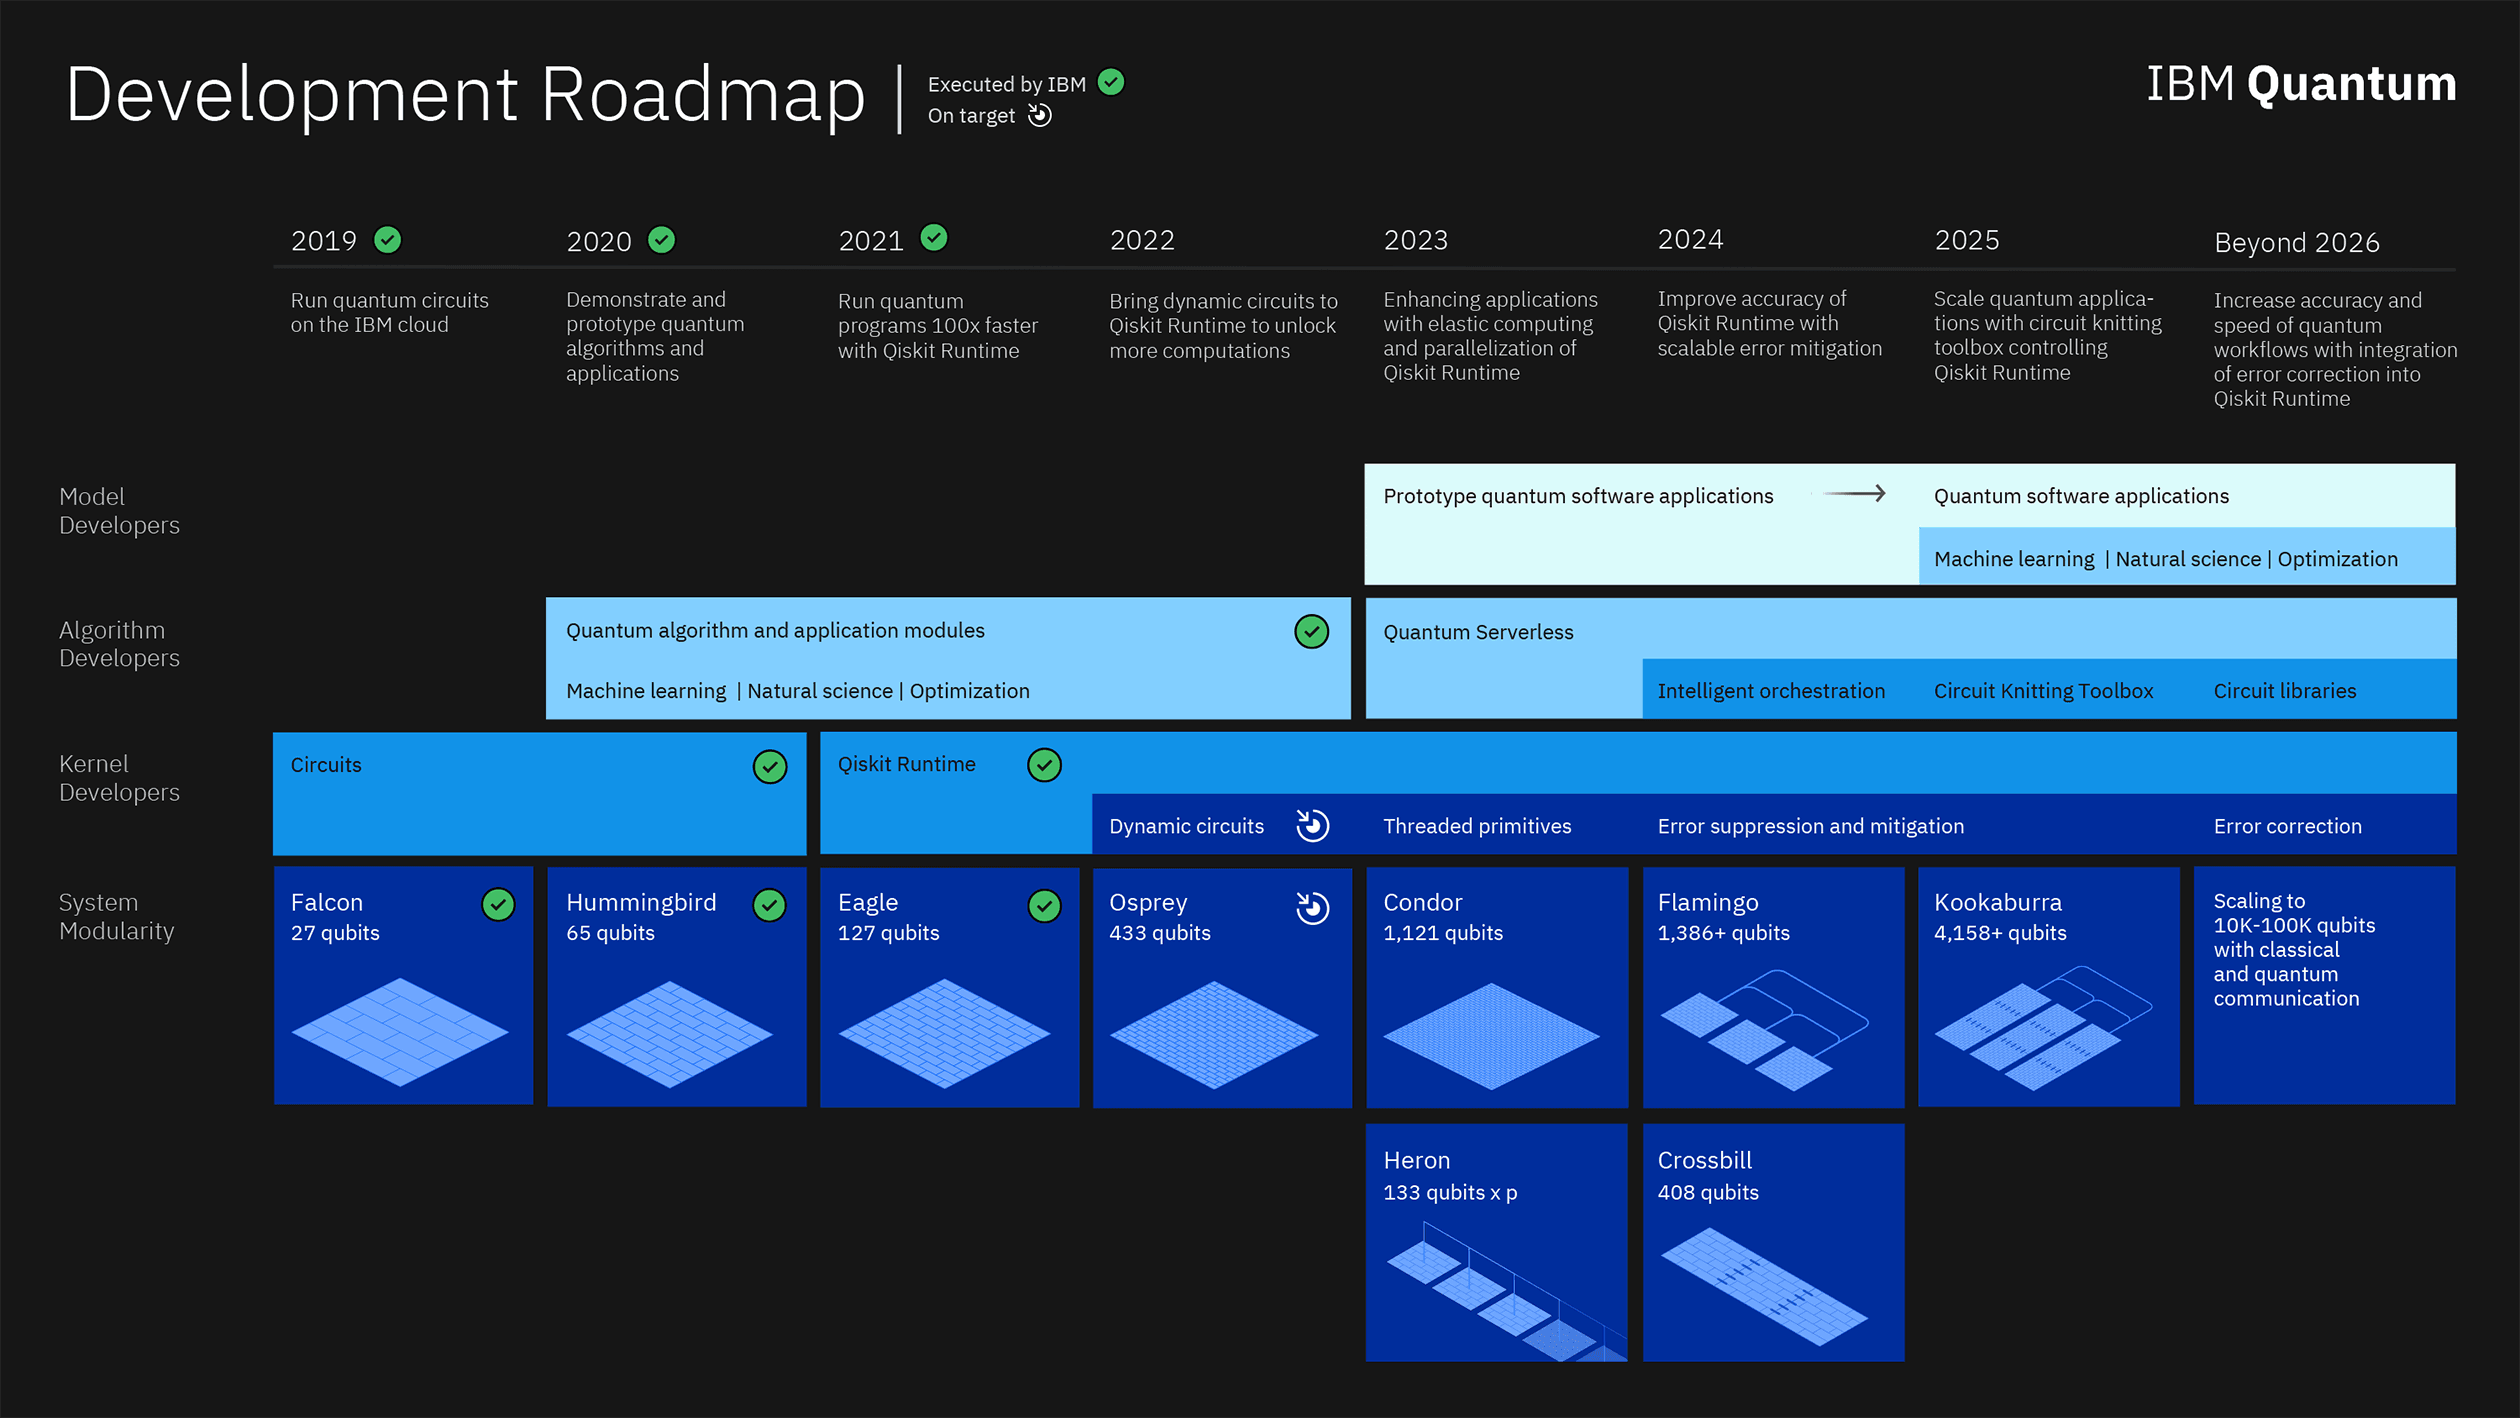
\includegraphics[width=\textwidth]{figures/IBM Roadmap.png}
  \caption{IBM quantum roadmap.} \label{IBM Roadmap}
\end{figure}
\begin{figure}[ht]
  \centering
  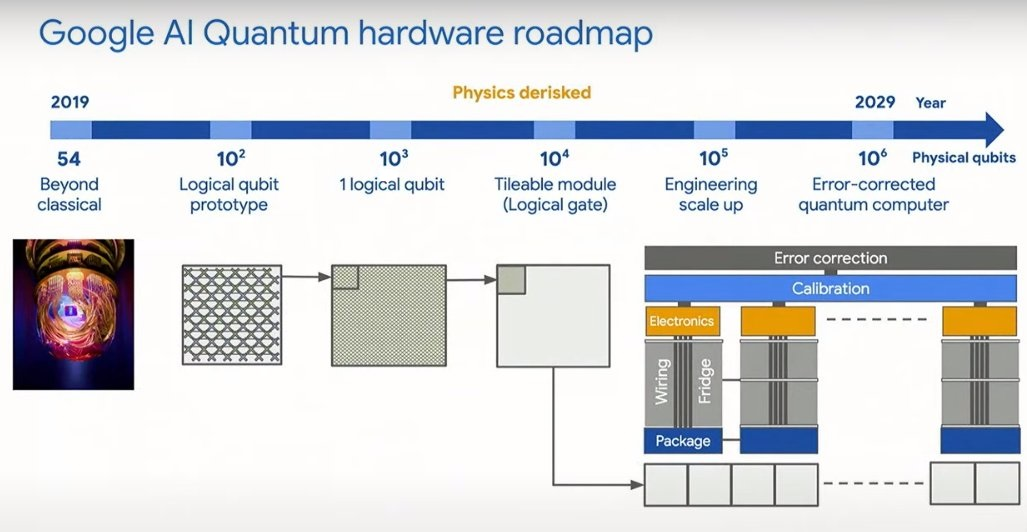
\includegraphics[width=\textwidth]{figures/Google quantum roadmap.jpg}
  \caption{Google quantum roadmap.} \label{Google quantum roadmap}
\end{figure}
\begin{figure}[ht]
  \centering
  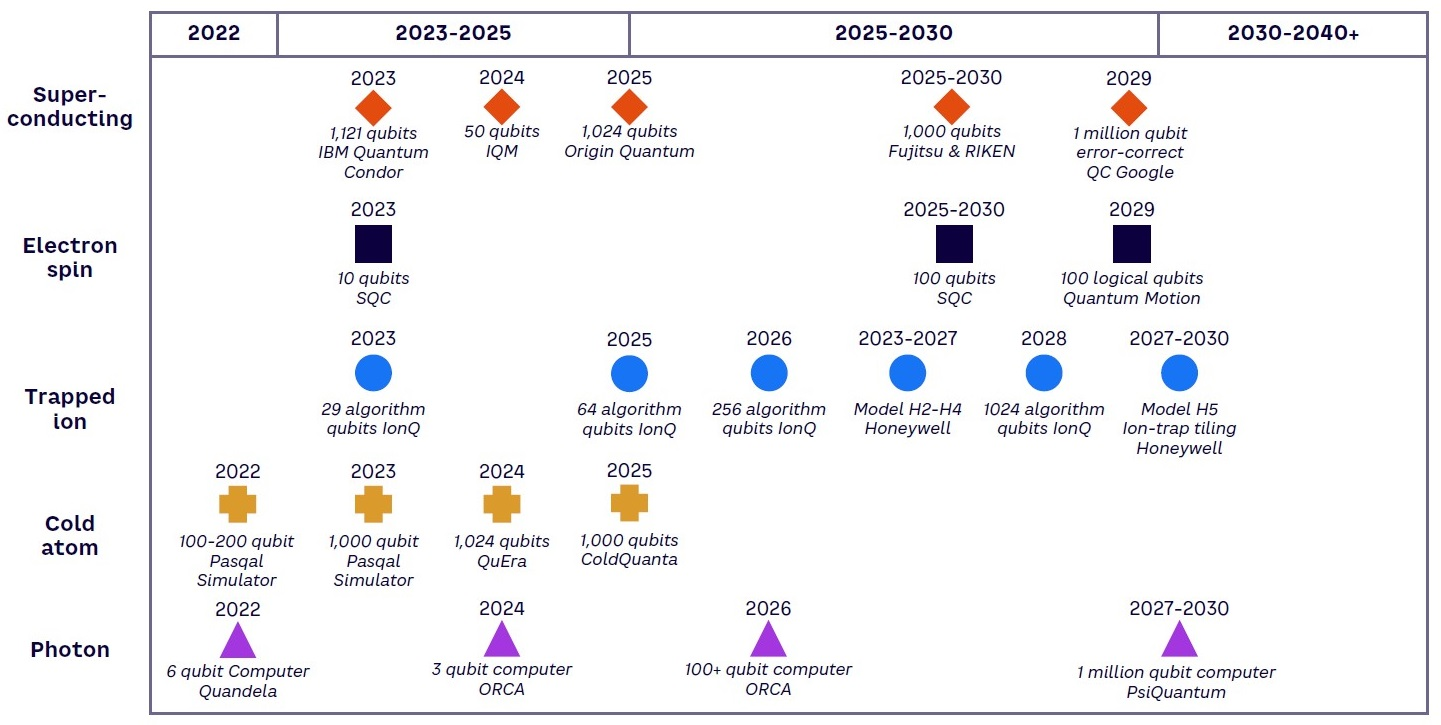
\includegraphics[width=\textwidth]{figures/Quantum computing roadmaps.jpg}
  \caption{Quantum computing prototypes announced on different roadmaps \cite{BibEntry2022May}.} \label{Quantum computing roadmaps}
\end{figure}

\section{Algorithms comparison}

\subsection{QPE and VQE}
By comparing the formulas in eq. (\ref{Scaling QPE}) and (\ref{Scaling QPE 1}) and eq. (\ref{Scaling VQE}) and (\ref{Scaling VQE 1}), or more precisely eq. (\ref{Scaling VQE 2}), we can see that the QPE algorithm is asymptotically more efficient than the VQE. \\
It scales linearly, with respect to the number of spatial orbitals, in both width and depth. It allows to achieve a higher precision with a lower computational cost in terms of depth, since it scales as $O(\frac{1}{\epsilon})$, while the VQE scales as $O(\frac{1}{\epsilon^2})$. The number of repetitions is a constant value that depends on the chemical system and this is the best result one can hope to achieve. \\
This leads to the conclusion that QPE is most likely the best quantum algorithm to simulate large-size molecules, i.e. molecules with hundreds or thousands of atoms. \\
However, as already expressed throughout the thesis, QPE also requires to work with logical qubits or equivalently fault-tolerant devices, which translates in long coherence time and number of physical qubits even for simulation of small-size molecules. Furthermore, a good approximation of the target wave function is needed, i.e. the fidelity of the input state to the unknown target eigenstate approaches one, thus using a randomized state as input is not an option as its expected fidelity to the target eigenstate approaches zero exponentially in the system size, resulting in QPE becoming exponentially costly with imperfect input state preparation. \\
The core component of QPE, however, is efficient Hamiltonian simulation and it is fundamental to study alternative methods to Trotterization that perform better in order to lower the computational requirements, especially in the depth of the circuit, i.e. gate count. In addition to that, researches on scalable quantum hardware, be it superconducting circuits, ion traps or other technologies, will enable increasingly large circuits both for calculation and error-correction schemes. \\
\\
The VQE, on the other side, trades off the depth and the number of qubits required under QPE with a higher number of measurements and repetitions of the circuit as well as with the constraints of an approximate ansatz for the state. Although this could result in a more efficient simulation for small-size molecules it is not a viable path, in other words, the VQE is not an efficiently scalable algorithm. \\
It is important to note that much lower number of shots would be sufficient to progress the initial part of the optimization and a high number is only required in the last iterations of a VQE close to convergence to reach chemical precision (however this number may need to be much higher in case of barren plateaus). \\
A solution which needs to be researched more thoroughly is the potential parallelization of the VQE. This is because parallelism of the VQE offers a direct way to convert runtime cost into hardware cost by splitting the shots required onto different sets of qubits, which can be arranged in different threads on a single quantum computer or multiple disconnected quantum computers. \\
However, there are many caveats to the potential of this method. First, parallel quantum computing suffer from communication overheads and secondly, parallelization could result in higher noise levels. \\
\\
While many other factors affect the overall time scaling of both methods, this point illustrates the asymptotic efficiency of QPE compared to VQE assuming access to fault-tolerant quantum computers, but also the resource efficiency of VQE over QPE for NISQ-era devices. \\
The frontier between NISQ and FTQC is blurry and as pointed out by Wang et al. \cite{Wang2019Apr} so is the frontier between VQE and QPE. They presented an interpolation between the two algorithms labeled accelerated VQE (or $\alpha$-VQE), which uses smaller scale QPE calculations as subroutines for the VQE. This method introduces a parameter $\alpha \in [0,1]$ which allows the tuning of the circuit depth $O(1/\epsilon^{\alpha})$ and the number of samples $O(1/\epsilon^{2(1-\alpha)})$. One recovers the QPE scaling if $\alpha = 1$ and the VQE scaling if $\alpha = 0$. \\
As a general perspective, rather than being mutually exclusive methods for solving an electronic structure problem, VQE and QPE are likely to provide the most benefit when combined as complementary approaches, offering algorithmic flexibility that can be adjusted depending on the progress of quantum hardware. This means, for example, that VQE can be used to implement the state preparation task of the QPE algorithm, this would make the overlap between the input state and the target eigenstate more prominent, it raises the probability of calculating the correct expected eigenvalue and correspondingly it lowers the number of repetitions of the entire QPE method, as we saw mathematically from eq. (\ref{Scaling QPE}) and (\ref{Scaling QPE 1}).

\subsection{Classical and quantum}
Most conventional approaches for high accuracy calculation of ground state energetic properties of molecular systems rely on wave function approximations, which we presented in Chapter \ref{Quantum computational chemistry}. These show a similarity with VQE, in which the focus of the algorithm is to best approximate the wave function by defining the single basis functions, which determines the resolution and the representation of the system. \\
This means that the most likely competitors for short to medium term applications of VQE are accurate wave function approaches, e.g. CC and CI methods, which, as we have described, scale as high polynomials or even combinatorially, but they are still able to access systems of comparable size. \\
\\
The largest conventional CI calculations which have been reported in the literature are proof-of-principle studies. They include \cite{Elfving2020Sep}:
\begin{enumerate}
    \item A calculation involving a complete active space (CAS), i.e. modelling the electrons in the partially occupied orbitals with all combinations of the Slater determinants with 20 electrons in 20 spatial orbitals (40 spin-orbitals), realized within the framework of the MCSCF method on a chromium trimer, corresponding to approximately $4.2 \cdot 10^9$ single determinants (SDs);
    
    \item A single point CASSCF calculation on a pentacene molecule with 22 electrons in 22 spatial orbitals (44 spin-orbitals), corresponding to approximately $5.0 \cdot 10^{11}$ SDs;
    
    \item A single iteration of the iterative CI algorithm for a chromium tetramer with 24 electrons in 24 spatial orbitals (48 spin-orbitals), $\sim 7.3 \cdot 10^{12}$ SDs.
\end{enumerate}
All these CI calculations utilized the 6-31G* basis set. To put the number of the SDs in chemical context a FCI calculation on the propene molecule in the minimal STO-3G and the larger, but still very small, 6-31G basis set would correspond to 24 electrons in 21 and 39 spatial orbitals (42 and 78 spin-orbitals), respectively. The frequently used frozen core (FC) approximation would reduce the number of active electrons in propene to 18, but already the next homolog, 2-butene, will have 24 active electrons in the FC approximation and push against the limits of the feasible FCI calculations. \\
\\
As for the CC method, describes in Chapter \ref{Quantum computational chemistry} that the CCSD(T) method treat dynamic correlation accurately and shows size extensivity (correct scaling with the system size) and size consistency (separability of energies for non-interacting fragments). \\
Among the largest CC calculations reported in the literature are \cite{Elfving2020Sep}:
\begin{enumerate}
    \item A CCSDT(Q)/cc-pVTZ single point energy calculation on benzene in the FC approximation (30 electrons, 264 basis functions) which corresponds to $\sim 3.1 \cdot 10^9$ single, double and triple as well as $\sim 2.2 \cdot 10^{12}$ perturbative quadruple t-amplitudes;
    
    \item The largest conventional CCSD(T) calculation ever performed is that by Yoo and co-workers on a (H$_2$O)$_{17}$ cluster in the aug-cc-pVTZ basis set, which corresponds to 128 electrons in the FC approximation and 1564 orbitals;
    
    \item A similar (H$_2$O)$_{16}$ calculation had to be executed on 120 000 computer cores and took more than 3 hours;
    
    \item Another notable CCSD(T) effort is that of Gyevi-Nagy and co-workers in which the energy of 2-aminobenzophenone (ABP, C$_{13}$H$_{11}$NO) was computed in the large def2-QZVPPD basis set. That calculation, utilizing the density-fitting approximation, correlated 90 non-FC electrons among 1569 orbitals and was completed on 224 computer cores in 68 hours.
\end{enumerate}
VQE has an advantage over classical methods since in its circuit it implements an ansatz that can approximate a wide range of wave functions. To put it another way, it analyzes a big portion of the Hilbert space derived by the qubits register, which ultimately corresponds to the number orbitals of the chemical compounds. An example of this result is the UCC ansatz, which was already described by Peruzzo et al. \cite{Peruzzo2014Jul} as a modelization that has no efficient implementation on a classical computer but it has one on a quantum computer. \\
VQE does so with a scaling in computational requirements which competes with the one of high accuracy classical methods, both in width and in depth. We can see that from eq. (\ref{classical scaling}) and eq. (\ref{Scaling VQE}) and (\ref{Scaling VQE 1}) or eq. (\ref{Scaling VQE 2}) or otherwise from Figure \ref{Accuracy vs Computational resources}. \\
Taking the results from Gonthier et al. \cite{Gonthier2020Dec}, described in Chapter \ref{Quantum computing for computational chemistry: NISQ devices}, focusing on the scaling of $b$ from Figure \ref{K values} and omitting the prefactor $a$, the results for the basis rotation grouping technique suggest that VQE has the potential to scale better with system size than methods such as CC. \\
The expressivity and the better scaling can result in a computational advantage, but we need to consider two restrictions to define this advantage. First, VQE must demonstrate similar or higher accuracy than any conventional method but with lower computational time-to-solution. This condition takes into account possible limitations due to hardware runtime, potentially resulting in a large prefactor for VQE computations. If the VQE has better asymptotic scaling than conventional methods, but a large prefactor, this means an advantage could only be achieved in the asymptotic regime of very large systems, with runtime possibly too large for VQE to be realistically usable. This would make it difficult to demonstrate quantum advantage for practical moderately sized systems. The second condition is to achieve at least as good accuracy, with faster compute time, for a system of sufficient complexity to accurately model a real problem of physical and chemical relevance. This involves demonstrations on systems where the approximation error in defining the specific Hamiltonian for the original problem is of smaller magnitude than its solution using the VQE. This could be as simple as ensuring that basis sets are sufficiently saturated or that the complexity of the interactions with a wider system were sufficiently resolved. For instance, consider computing the energy of a series of protein-ligand complexes: even if the VQE achieves better accuracy in lower computation time, it is not guaranteed that these accuracy gains lead to a practical advantage. \\
\\
These methods all aim to simulate small-size molecules with high accuracy. If instead we want to analyze large-size and industrially relevant compounds, especially in the case of complex heterogeneous materials, the great majority of first-principles simulations are conducted using density functional theory, which, as shown in Chapter \ref{Density functional theory}, is in principle exact but in practice requires approximations to enable calculations. Within its various approximations DFT has been extremely successful in predicting numerous properties of solids, liquids, and molecules and in providing key interpretations to a variety of experimental results. However, it is often inadequate to describe strongly-correlated electronic states. \\
The boundary between strongly correlated and weakly correlated is imprecise from a quantitative point of view, but one may use the definition that a weakly-correlated system is one for which chemical accuracy can be obtained by coupled-cluster theory with single and double excitations and a perturbative treatment of connected triple excitations, CCSD(T), and a strongly-correlated system is one that requires higher excitations for chemical accuracy. This issue is particularly prevalent when two or more configurations are nearly degenerate. For this reason, strong correlation is often called near-degeneracy correlation. \\
\\
For strongly-correlated systems the main difficulty lies in the size of the active spaces required for correctly describing them. This is because individual electron-electron interactions determine the behaviour of the whole system and they lead to complex structures that need high accuracy on a local scale, while methods like DFT or force fields (a method that model forces and bonds between atoms in a classical Newtonian parametrization) give results that are too approximative. This is particularly true for materials science, where systems, i.e. materials, consists of hundreds or thousands of atoms arranged in lattices which mostly interact locally through individual electrons or pair of electrons, e.g. superconductors. \\
Moreover, as we mentioned before, DFT can not be systematically improved, but one has to define a different functional for each simulated system. This can make the method impractical because it introduces empirical parameters that bind the result of the simulation to the experimental capabilities, which is the opposite of why a simulation method is used, that is, for the inference of chemical properties. \\
In this condition QPE shows an advantage over classical methods since it leads to highly accurate results. That is because, as we described, it considers the system in a full quantum way, both in the definition of the wave function and in the implementation of the evolution through direct interactions between all the components. \\
\\
For weakly-correlated large-size systems, for example drug molecules that interact with proteins, researched by the pharmaceutical industry, the methods aim to simulate an environment of hundreds of thousands of atoms. This makes the full quantum mechanical treatments of such systems out of reach. As a consequence, the most widely used computational techniques in pharma rely on force fields. However, while classical force fields capture most prominently bond lengths, bond angles, dihedrals as well as non-bonded electrostatic and van-der-Waals interactions, their traditional formulation does not account for finer electronic effects such as polarization, charge-transfer phenomena, aromatic stacking interactions or interactions with metal ions. \\
Thus, when more accurate treatment is required the approach that is traditionally used to describe the system is a hybrid method: a quantum mechanical (QM) technique is used to describe selected residues of the binding pocket and the drug, while the remainder of the system is simulated using molecular mechanics (MM). This is called QM/MM method. \\
QPE can bring to an advantage in this context, that is because of its asymptotic scaling. We can see that from eq. (\ref{classical scaling}) and eq. (\ref{Scaling QPE}) and (\ref{Scaling QPE 1}) or otherwise from Figure \ref{Accuracy vs Computational resources}. QPE can produce all the configurations in the Hilbert space generated by the qubits register and elaborates them in linear scaling width and depth. \\
Again simulation algorithms on quantum computers have a higher expressivity due to the intrinsic nature of the technology used to perform the calculation, but to prove a real quantum advantage the method must not introduce a significant overhead compared to classical methods, so that the improvements in the accuracy of results will come at a reasonable cost. This is why the main research on QPE revolves around finding an alternative core component to Trotterization that can lead to lower computational requirements.

\section{Targets of simulation}

\subsection{Defining advantage}
Quantum advantage in computational chemistry can be sought in a space of three dimensions: speed, accuracy, and molecule size. These define advantages that are not useful in practical or industrial applications \cite{Elfving2020Sep}:
\begin{enumerate}
    \item \textbf{Irrelevance due to availability of accurate experimental results} \\
    These are the cases where quantum computers would have to compete with experimental measurements that are accurate, fast, inexpensive and straightforward. It is obvious that in presence of readily available and reliable experimental data there is little need for simulated results;
    
    \item \textbf{Irrelevance due to availability of conventional computational results} \\
    These pertains to chemical systems or problems for which quantum chemical calculations on classical computers can produce chemical accuracy results in little time (seconds, minutes or even a few hours). These are exactly the types of applications on which quantum computing algorithms have been routinely validated so far;
    
    \item \textbf{Irrelevance due to real world complexity} \\
    Often the biggest problem in simulation research is not simply to complete single computations in reasonable time with sufficient accuracy. When simulated chemical processes are very complicated and involve potentially hundreds of intermediates, conformations or reaction paths, as in catalytic and metabolic pathways, the real research bottleneck lies in a combinatorial explosion of possibilities to probe with simulation. In such projects, even if the calculations themselves became orders of magnitude faster or more accurate, for example, through the exploitation of quantum computing, the whole project might enjoy only a modest speedup;
    
    \item \textbf{Irrelevance to industrial applications} \\
    These are molecular systems that, even if described accurately on a quantum computer, are likely to remain academic and theoretical interest and fail to lead to transformative changes in chemistry.
\end{enumerate}

\subsection{Applicability forecast}
Now we focus on how the molecular size affects the capability of quantum computers to simulate molecular systems. \\
Despite the general impracticality of the largest calculations mentioned above, just the sheer fact that they have been accomplished on classical computers sets the bar very high for quantum computers. \\
The size of ABP, mentioned in the last section, makes it an attractive minimum viable system in real world practical applications. Systems of this size are regularly used for parameterizing force fields in areas of research like computational drug design. \\
\\
We saw that accuracy is strictly linked to the basis set and especially on the number of functions chosen to model the system. \\
To give an example of the relation between basis sets and accuracy we take two simple molecules, the H$_2$ and He molecules. For these one does not achieve chemical accuracy at the FCI level with the cc-pVTZ basis set (28 basis functions or 56 spin-orbitals). One has to use either cc-pVQZ or both cc-pVDZ and cc-pVTZ in an extrapolation scheme for H$_2$, whereas for He at least the cc-pVTZ (14 functions or 28 spin-orbitals) and cc-pVQZ (30 functions or 60 spin-orbitals) basis set energies are required as inputs to an extrapolation scheme. \\
However, in recent experiments with quantum computing hardware, applied to simulating molecular and materials chemistry, the number of qubits that have been used is significantly smaller than the one necessary to achieve chemical accuracy, for all molecules studied. Experiments are shown in Figure \ref{Experiments with quantum computers}. \\
\begin{figure}[ht]
  \centering
  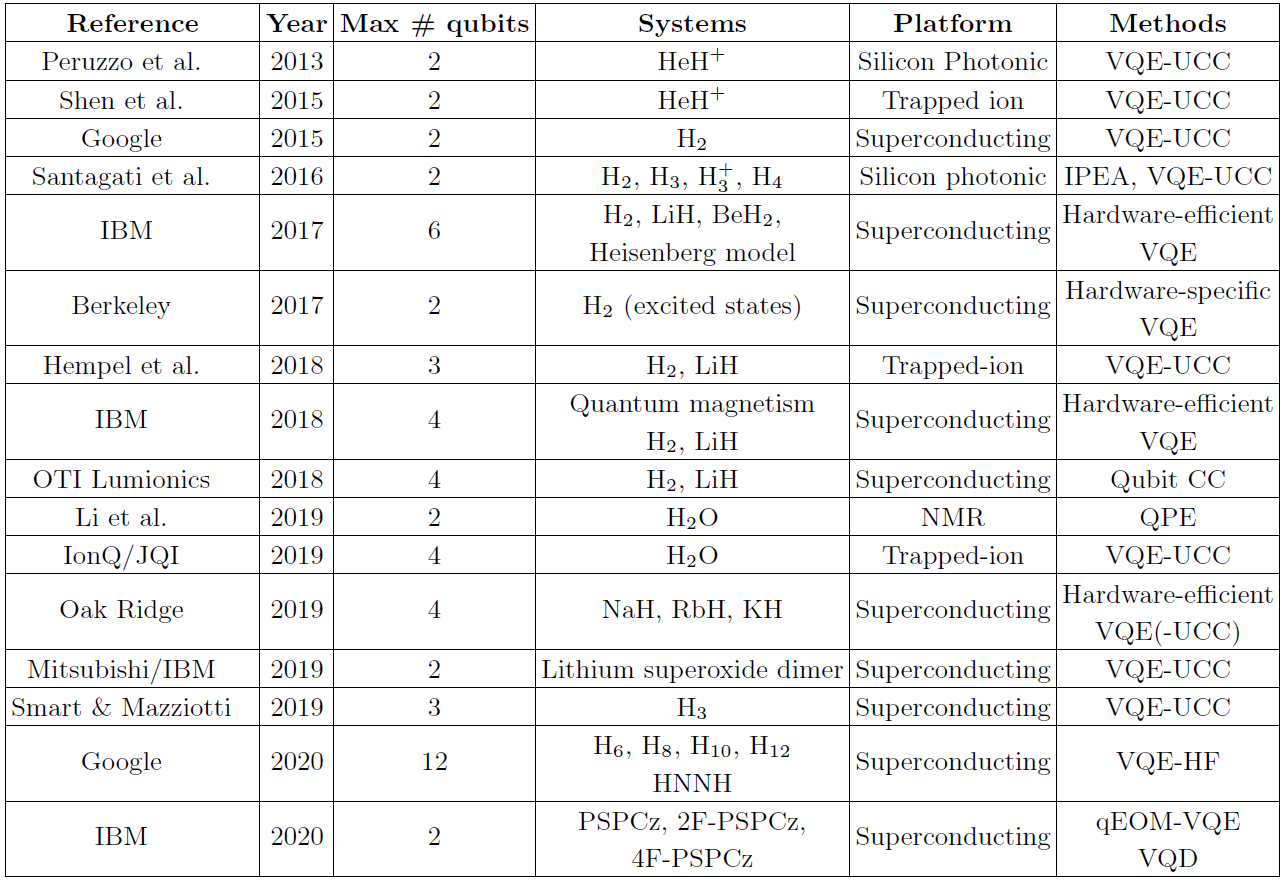
\includegraphics[width=0.95\textwidth]{figures/Experiments with quantum computers.png}
  \caption{Simulations on real quantum computers \cite{Elfving2020Sep}.} \label{Experiments with quantum computers}
\end{figure} \\
Moreover, in 2021 Huggins et al. \cite{Huggins2022Mar} simulated a simplified version of the energy state of a molecule consisting of 12 hydrogen atoms with 12 qubits, each one representing one atom’s single electron. They then modeled a chemical reaction in a molecule containing hydrogen and nitrogen atoms, including how that molecule’s electronic structure would change when its hydrogen atoms shifted from one side to the other. That represents "the largest chemistry simulations performed with the help of quantum computers". \\
\\
Elfving et al. \cite{Elfving2020Sep} proposed the chromium dimer, Cr$_2$, as a good target for benchmarking simulation on quantum computers. This molecule, with its very short formally sextuple bond and a peculiarly shaped dissociation curve, could be a critical test for electronic structure methods. \\
In their calculation on this target they chose the complete active space (CAS) approach, where they selected an increasing number of active orbitals and active electrons. The notation used to define the number of electrons and the number of orbitals used in the model is (N, N). They carried on a resource estimation on ground state energy estimation, focusing especially on the core component of QPE algorithm and comparing Trotterization and qubitization methods with surface code for error-correction. \\
This comparison is brought with reference to the number of T and Toffoli gates, i.e. the depth, and the number of logical qubits, i.e. the width. They showed that quibitization, especially in its sparse form, gives rise to a relatively large overhead in the number of logical qubits but it is optimized in terms of the non-Clifford gate complexity, leading to the conclusion that the trade-off between Trotterization and qubitization is the circuit depth versus the number of logical qubits. \\
After that, they compared the result on the quantum computer, in terms of wallclock time scaling, to a desktop PC simulation (corresponding to a Intel i9-10980XE, with $\sim$1.2 TFLOPS) and a 10$^5$x faster extrapolation (corresponding to a top-5 HPC, at $\sim$125 PFLOPS). The results are shown in Figure \ref{Runtime chromium dimer} and \ref{Resource estimates chromium dimer}. They considered error rates $p=10^{-3}$ (already achieved in experiment) and $p=10^{-6}$ (long-term hardware ambition).
\begin{figure}[ht]
  \centering
  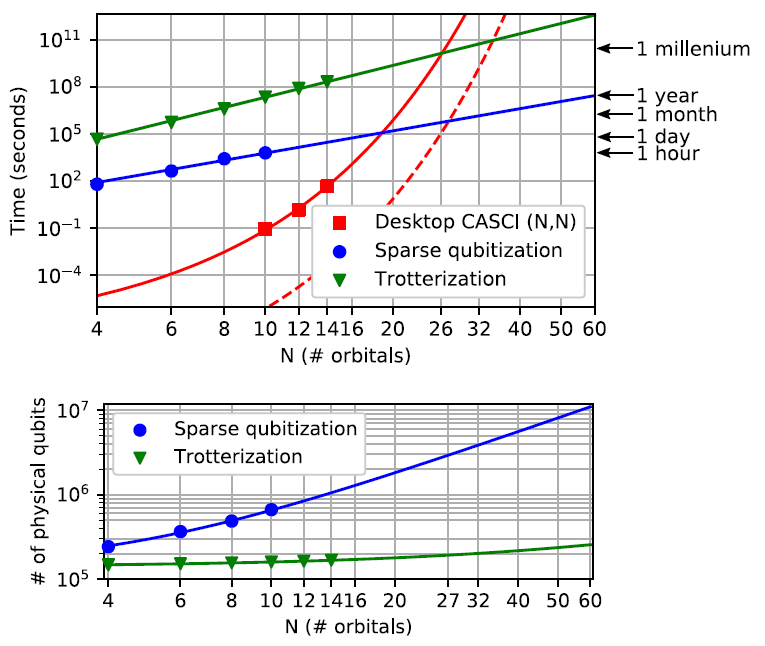
\includegraphics[width=0.8\textwidth]{figures/Runtime chromium dimer.png}
  \caption{Runtime and physical qubit requirements for the chromium dimer (Cr$_2$) \cite{Elfving2020Sep}.} \label{Runtime chromium dimer}
\end{figure} \\
\begin{figure}[ht]
  \centering
  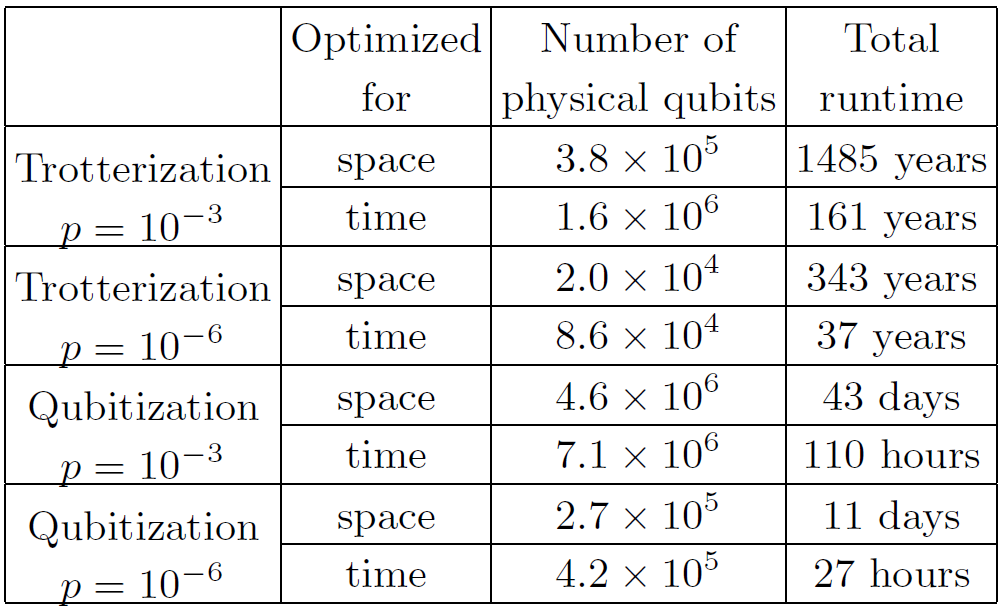
\includegraphics[width=0.7\textwidth]{figures/Resource estimates chromium dimer.png}
  \caption{Resource estimates for simulating the chromium dimer with a CAS space of (26,26) \cite{Elfving2020Sep}.} \label{Resource estimates chromium dimer}
\end{figure} \\
The figures show that the approximate size where a quantum computer solves the problem faster than a classical computer is for a (N, N) CAS size of around N = 19 - 34. For N $>$ 34 any of the assessed quantum algorithms should be faster than any available classical computer. N = 19 implies a physical qubit count of $\sim 10^5$ for Trotterization and $\sim 3 \cdot 10^6$ for sparse qubitization. However, in the case of Trotterization the crossover point happens at a total runtime approaching a thousand years, which even with some optimization operations seems infeasible. The crossover for qubitization appears to happen at approximately the same point as the maximum size which is still feasible at all on a classical supercomputer. \\
Although the resource estimates give an indication of the current state of the art in algorithms, these are not necessarily lower bounds and simulation algorithms may improve by orders of magnitude both in terms of complexity and prefactor. \\
This makes it possible to delineate a range of possible targets of application for algorithms on quantum computers. In Figure \ref{Targets of simulation} we show a scheme of the molecule systems with resepect to the number of spatial orbitals used to carry on a simulation in the CAS approach. \\
\begin{figure}[ht]
  \centering
  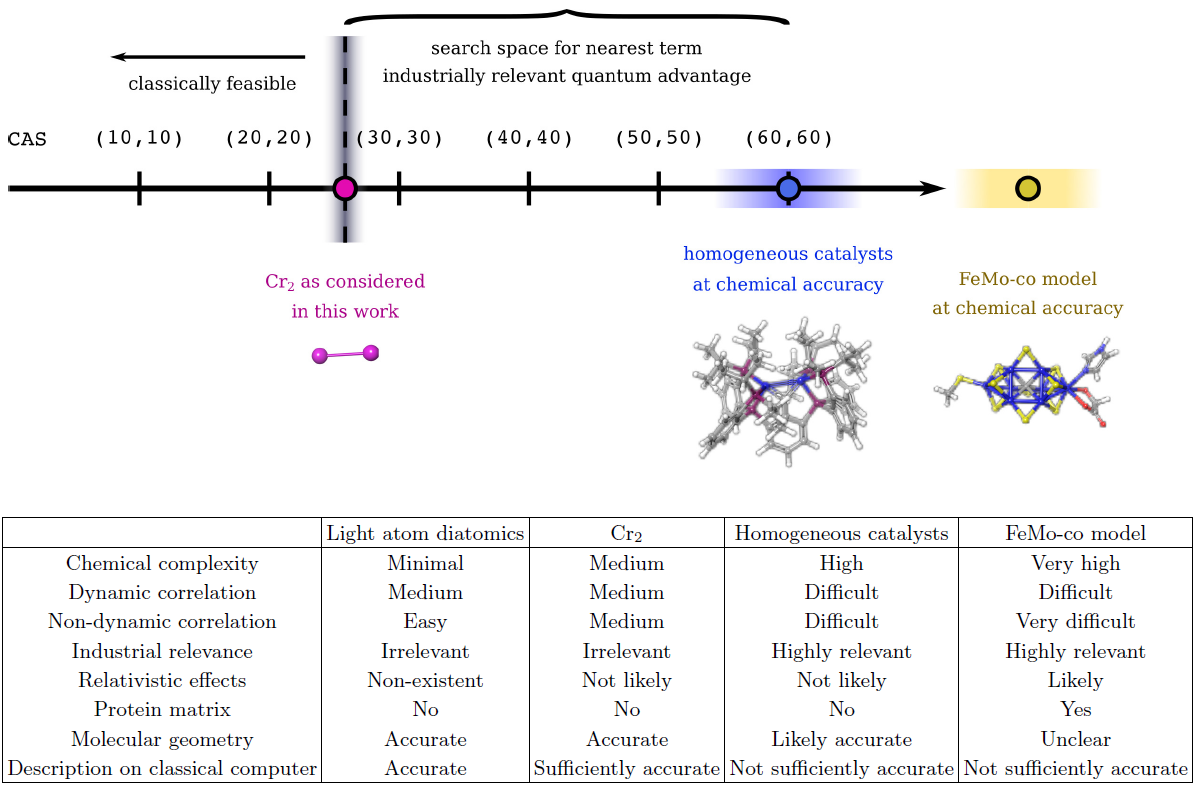
\includegraphics[width=\textwidth]{figures/Targets of simulation.png}
  \caption{Possible short term quantum computer applications and schematic placement of their CASs \cite{Elfving2020Sep}.} \label{Targets of simulation}
\end{figure} \\
Light atom diatomics are not put on the CAS axis because of the unclear boundaries between the dynamic and non-dynamic correlation in these molecules. The use of these methods for small molecules containing only light atoms, which have been an object of study and research direction in most of the quantum computing literature, does not appear to be promising. \\
On the other side of the spectrum are large and complicated molecules, the properties and chemistry of which stand little chance of being accurately described by classical computers. An example of such a molecular system is the FeMoco protein system. Although very relevant for possible industrial applications, FeMoco presents an overwhelming complexity for a short-term quantum computer. \\
For a relevant successful application of quantum computations a "sweet spot" lies somewhere in the middle between tiny light atom molecules and large complex multi-metal active sites of protein complexes. \\
\\
The chromium dimer molecule, lacking industrial applications, can not be regarded as a good ultimate target for quantum computers, but it can be used as a model or rather as a testing ground on a way to the middle ground system to seek. One type of chemistry for such a middle ground can be found among medium-sized inorganic catalyst molecules which are a subject of homogeneous catalysis research. A report \cite{vonBurg2021} investigated the applicability of quantum algorithms to the quantum chemical description of a ruthenium-containing catalyst designed to convert CO$_2$ into methanol. The authors proposed the treatment of active spaces that span 48-76 electrons and 52-65 orbitals. An attractive subclass of homogeneous catalysts on which early quantum advantage studies can be focused are biomimetics. These normally di- and tri-metal complexes borrow chemical insight from natural metal-containing enzymes and are designed for tackling industrially important chemical transformations such as C-H bond activation or the N$_2$ bond cleavage. Highly efficient C-H bond activation, for example, is at the heart of the idea of "methanol economy", which seeks to replace petroleum and coal by cleaner sources of energy and synthetic materials. \\
The estimates for the chromium dimer places quantum advantage for CASs of the structure (N, N) in the region after N $\approx$ 26. There is a gap between this value after which the quantum advantage can be expected and N $\approx$ 60, which is required for the accurate treatment of the non-dynamic correlation of homogeneous catalysts. The estimates for the latter type of molecules indicate that their treatment will require at least thousands of logical qubits. \\
\\
Little is left for the VQE method. If we assume that one could reach CASCI levels of precision in a given basis set, by using a VQE method on a NISQ device with a linear circuit depth, one can estimate with similar assumptions as above, that tackling a (26, 26) CAS problem would take about 1 hour per VQE iteration. Although this runtime does not seem completely prohibitive, the range of assumptions made, prevents from drawing strong conclusions for practical and industrially relevant application. \\
Gonthier et al. \cite{Gonthier2020Dec} made an estimate from the extrapolation of results from their organic molecules benchmark set, leading to a total runtime of a few hours, which could allow for a full VQE optimization with considerable effort. The results are shown in Figure \ref{Extrapolated runtimes organic molecules}. However, Hamiltonian coefficients for heavier strongly-correlated atoms like Cr might be larger, which would result in larger values of $K$. Moreover, even if such a computation becomes possible, the transition to practically relevant advantage could require active spaces beyond 100 qubits. \\
\begin{figure}[ht]
  \centering
  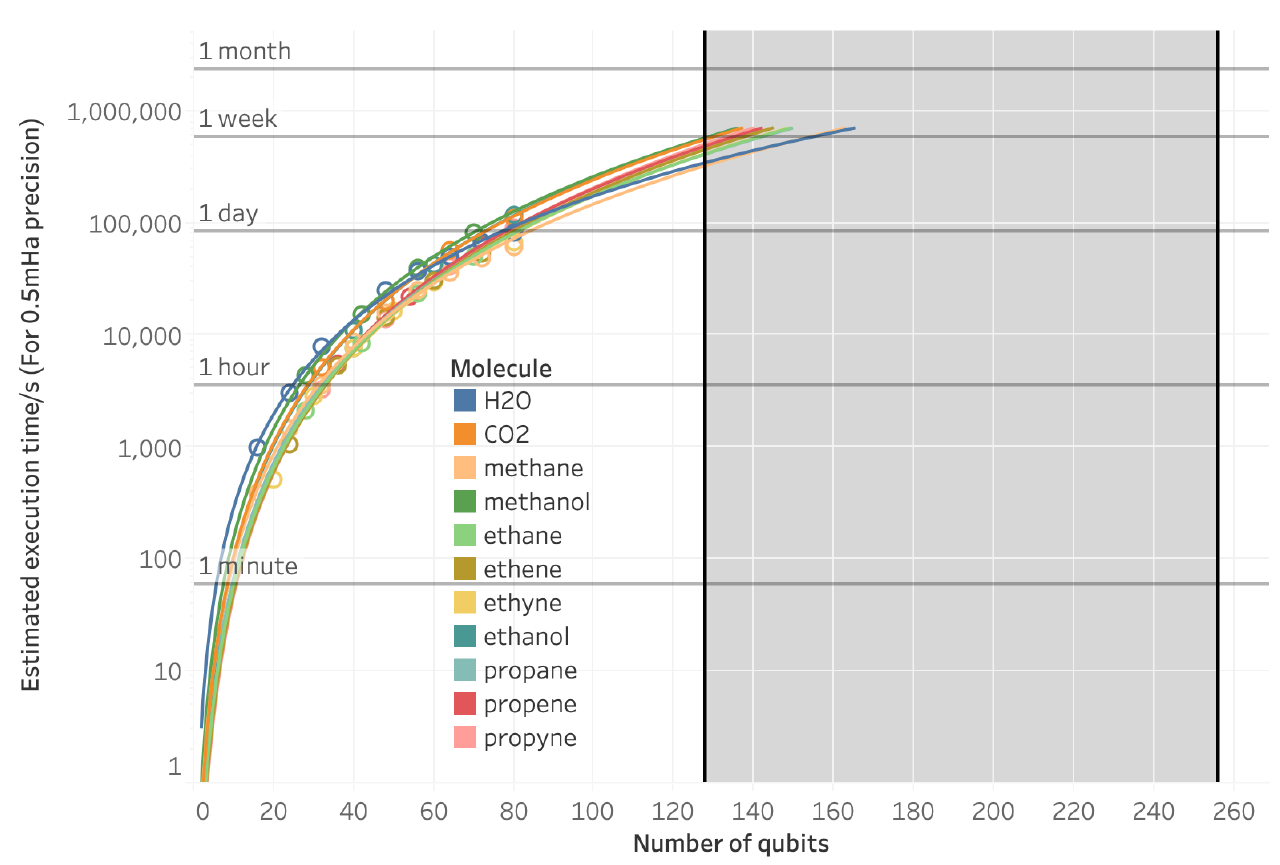
\includegraphics[width=0.95\textwidth]{figures/Extrapolated runtimes organic molecules.png}
  \caption{Extrapolated runtimes (in s) for the organic molecules benchmark set \cite{Gonthier2020Dec}.} \label{Extrapolated runtimes organic molecules}
\end{figure} \\
A more in-depth analysis of this problem has been made by Tilly et al. \cite{Tilly2021Nov} which provided the estimated runtimes for the steps in the VQE, included the general scaling for the chromium dimer, with an active space of 26 electrons in 26 molecular orbitals (52 spin-orbitals and 52 qubits). They compiled a 52 qubit version of k-UpCCGD assuming k = 1 and full connectivity of the qubit register. The results are shown in Figure \ref{Chromium dimer VQE}, where $L \sim 27 \ 000$ is the number of timesteps, i.e. the depth, $p = 170$ is the number of parameters, $T = 100$ ns is the assumed gate time, $P \sim 16N = 832$ is the number of operators and $S = 1/\epsilon^2 = $1 000 000 is the number of shots used for estimation. \\
\begin{figure}[ht]
  \centering
  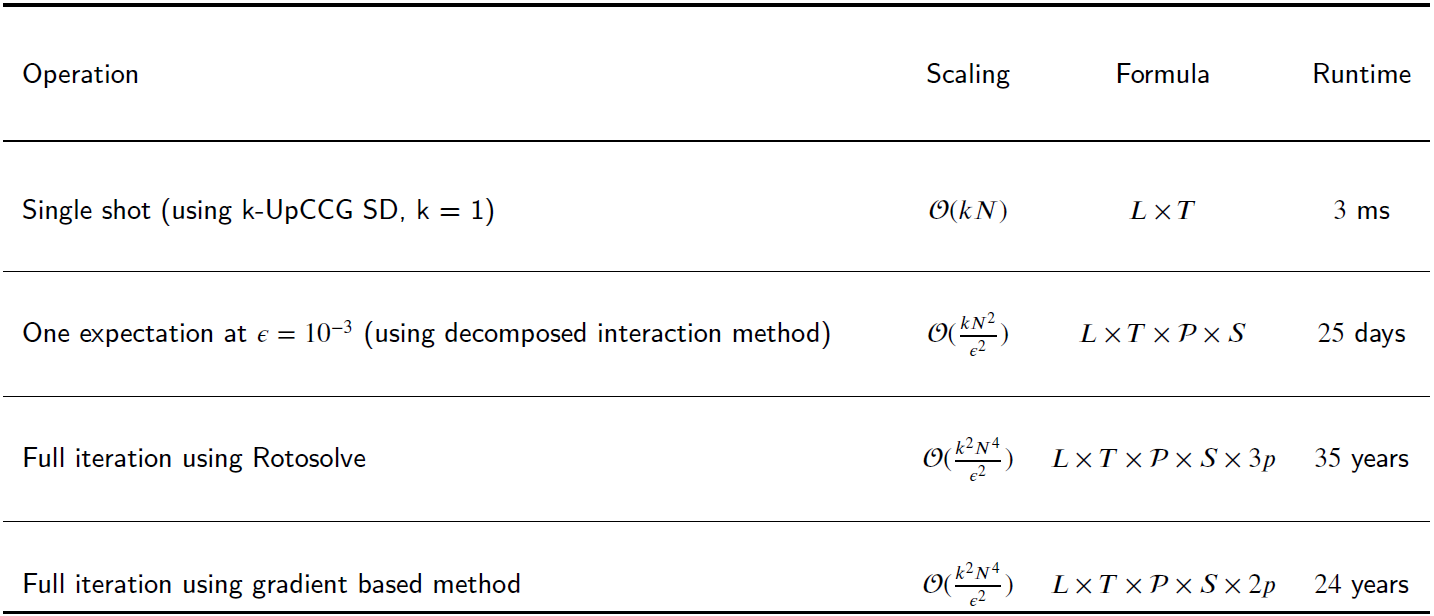
\includegraphics[width=\textwidth]{figures/Chromium dimer VQE.png}
  \caption{Estimates of one iteration of VQE for the simulation of the chromium dimer (Cr$_2$) molecule \cite{Tilly2021Nov}.} \label{Chromium dimer VQE}
\end{figure} \\
This demonstrates what we have already analyzed before in this chapter: the VQE will likely not show any advantages for practical and industrially relevant systems. \\
\\
Elfving et al. \cite{Elfving2020Sep} stressed that the real challenge is going from 10 to a million physical qubits, i.e. building a scalable platform, with logical qubits that can carry information and can be manipulated for virtually an infinite amount of time. \\
From a technological perspective this means that the next most important challenge to use these methods is to improve qubit error rates and error-correction codes. This is the approach that companies like Google (Figure \ref{Google quantum roadmap}) are pursuing and it is an unavoidable step for quantum computers to mature in their development. \\
This leads to the conclusion that the number of qubits alone is not a sufficient technological parameter to determine the quality of a real simulation. A precise forecast of applicability and improvability must take into account progresses in other parameters like maximum depth of a quantum circuit, $T_1$ and $T_2$, as well as quality parameters like quantum volume, precedently described. \\
A forecast based on available roadmaps is that in the next 1 to 3 years quantum processors with hundreds to a thousand qubits and high-fidelity connectivity will be built. This will be the crucial period for the development of error-correction codes and first logical qubits, as well as first software applications on NISQ devices. Then, if quantum communication and scaling techniques for these structures will be ready, comprising a lower error rate, between 4 to 6 years from now quantum processors with thousands to hundreds of thousands of physical qubits and roughly tens to a hundred logical qubits will be available and it will be possible to test the first defined targets for computational advantage. After that, in 7 to 9 years it is expected to reach structures of up to a million physical qubits and hundreds to a thousand logical qubits. This will be the minimum necessary computational capablity to provide computational advantages in practical and industrially relevant systems, as analyzed earlier in this chapter. \\
A more conservative forecast would be that the key milestone of achieving fault-tolerant large-scale quantum computers might occur in longer time, thus extending the period of their deployment to 10-15 years from now. \\
The technology development path at this limited level of maturity and with this level of complexity is unlikely to be linear. It is likely that a breakthrough will happen in the medium term and then the technological growth will be exponential. \\
As Niels Bohr said: "Prediction is very difficult, especially if it's about the future".

\section{Next steps}
In the last section of this thesis we show some of the possible next steps in the research for quantum computational chemistry. We focus especially on methods and targets of simulation.

\subsection{Problem fragmentation}
To tackle complex chemistry and material science problems using NISQ computers one can search for methods to reduce the number of electrons treated explicitly at the highest level of accuracy. Building on the idea underpinning dynamical mean field theory (DMFT), one may simplify such problems by defining active regions or building blocks with strongly-correlated electronic states, embedded in an environment that may be described within mean-field theory. \\
These methods goes under the name of 'problem fragmentation' or 'problem decomposition', another example is density matrix embedding theory (DMET). \\
\\
Ma et al. \cite{Ma2020Jul} proposed a quantum embedding theory built on one side on DFT, which is scalable to large systems and which includes the effect of exchange-correlation interactions of the environment on active regions, and on the other side on effective Hamiltonian for the active regions themselves using QPE or VQE. A general representation of this method is shown in Figure \ref{Quantum embedding theory}.
\begin{figure}[ht]
  \centering
  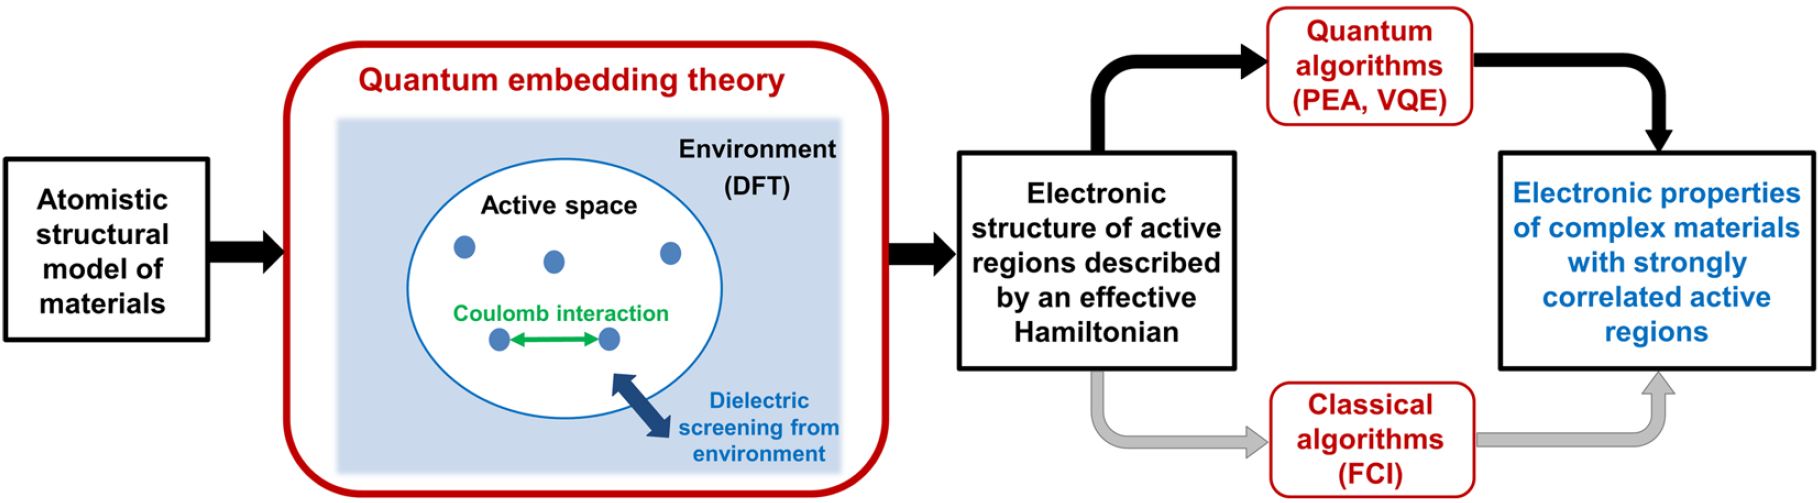
\includegraphics[width=0.95\textwidth]{figures/Quantum embedding theory.png}
  \caption{Quantum simulations of materials using quantum embedding theory \cite{Ma2020Jul}.} \label{Quantum embedding theory}
\end{figure} \\
The theory, inspired by the constrained random phase approximation (cRPA) approach, does not require the explicit evaluation of virtual electronic states, thus making the method scalable to materials containing thousands of electrons, and goes beyond RPA by explicitly including exchange-correlation effects. \\
The key part is to define the effective Hamiltonian
\begin{equation}
    H^{{\rm eff}} = \sum^A_{i,\alpha} t^{{\rm eff}}_{i\alpha} a^\dagger_i a_\alpha + \frac{1}{2} \sum^A_{i>j,\alpha>\beta} V^{{\rm eff}}_{ij\alpha\beta} a^\dagger_i a^\dagger_j a_\alpha a_\beta
\end{equation}
and consequently the effective kinetic ($t^{{\rm eff}}$) and potential ($V^{{\rm eff}}$) terms. These terms are one- and two-body interaction terms that take into account effect of all the electrons that are part of the environment in a mean-field fashion, at the DFT level. \\
An active space can be defined, for example, by solving the Kohn–Sham equations of the full system and selecting a subset of eigenstates among which electronic excitations of interest take place, e.g. defect states within the gap of a semiconductor or insulator. \\
They computed ground and excited state properties of several spin-defects in solids including the negatively charged nitrogen-vacancy (NV) center, the neutral silicon-vacancy (SiV) center in diamond, and the Cr impurity (4+) in 4H-SiC. Especially the investigation of the strongly-correlated electronic states of the NV center in diamond showed that quantum simulations yield results in agreement with those obtained with classical FCI calculations. \\
This method is similar to the one used by Reiher et al. \cite{Reiher2017Jul} in the experiment described in Chapter \ref{Quantum computing for computational chemistry: FTQC devices}, where the structure of the MoFe protein and the FeMoco active site are treated separately. \\
It could be essential to pursue this research for modelization and simulation of large-size systems like proteins.

\subsection{Materials science}
Throughout the thesis we focused especially on chemical systems as targets of quantum simulation methods, but systems and models which pertain to materials science could also be prominent targets of applicability. \\
These are mostly studied using lattices structures and plane wave basis sets. Their models all give rise to Hamiltonians with local interactions, thus efficiently simulatables on quantum devices. Moreover, large crystalline materials all exhibit quantum properties intrinsically related to the high level of correlation amongst their composing electrons \cite{Bassman2021Sep}. \\
Computing electronic band structures and phase diagrams to better understand these strongly correlated materials are grand challenges of condensed matter physics and materials science. This challenge is motivated both by practical considerations, such as the design and characterisation of novel materials, and by fundamental science. \\
\\
Stanisic et al. \cite{Stanisic2021Dec} showed experimentally how to implement an efficient quantum algorithm for simulation of the Fermi-Hubbard model. This is the simplest system that includes non-trivial correlations not captured by classical methods. Although it is a highly simplified model of interacting electrons in a lattice, to date the largest Fermi-Hubbard system which has been solved exactly consisted of just 17 electrons on 22 sites. \\
The Hamiltonian is defined as
\begin{equation}
    H = -\sum_{\langle i,j \rangle, \sigma} (a^{\dagger}_{i\sigma} a_{j\sigma} + a^{\dagger}_{j\sigma} a_{i\sigma}) + U\sum_i n_{i\uparrow} n_{i\downarrow}.
\end{equation}
In their experiment they used a low-depth VQE implementation with few parameters to simulate 1$\times$8 and 2$\times$4 instances on the Rainbow superconducting quantum processor in Google Quantum AI's Sycamore architecture with 23 qubits available. In Figure \ref{Qubit layout Fermi-Hubbard} the qubit layout used is shown. \\
In the quantum circuit to be optimized, the number of ansatz layers scales like the number of sites, corresponding to several hundred layers of two-qubit gates. While substantially smaller than previous quantum circuit complexity estimates for post-classical simulation tasks, this is still beyond the capability of today's quantum computers. \\
They achieved accurate representations of the ground state of Fermi-Hubbard instances beyond classical exact diagonalization and observed physical properties expected for the ground state, such as the metal-insulator transition, Friedel oscillations, decay of correlations and antiferromagnetic order.
\begin{figure}[ht]
  \centering
  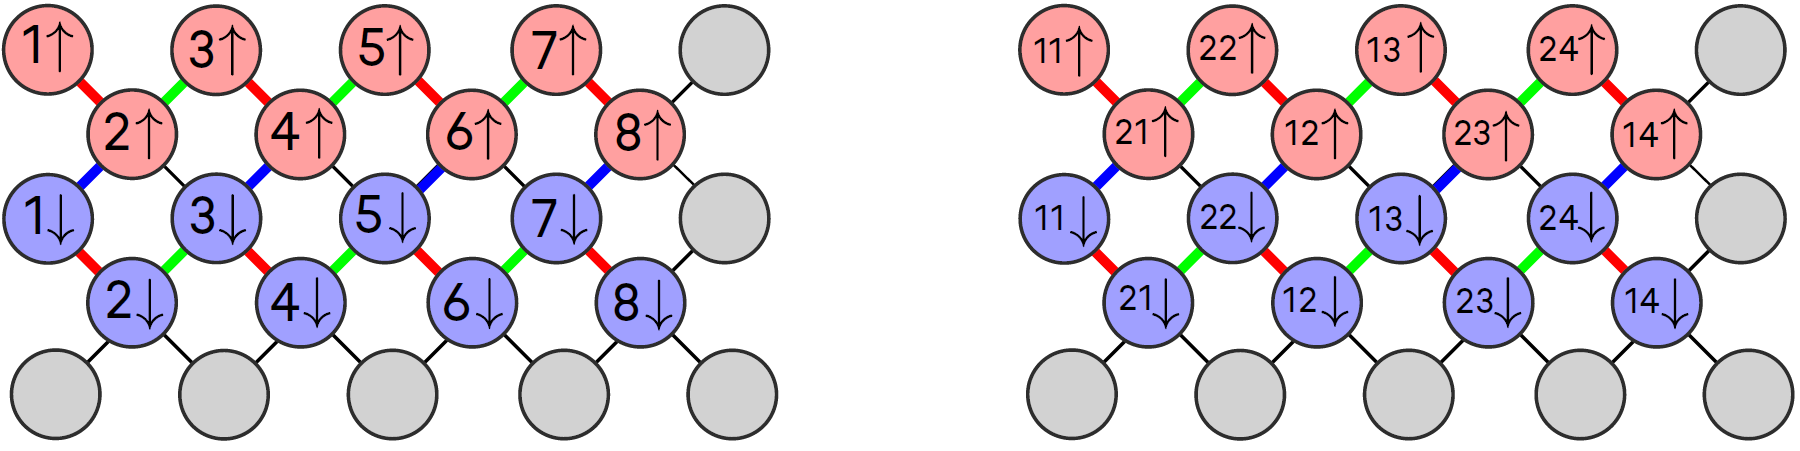
\includegraphics[width=\textwidth]{figures/Qubit layout Fermi-Hubbard.png}
  \caption{Qubit layout for implementing 1$\times$8 (left) and 2$\times$4 (right) Fermi-Hubbard instances \cite{Stanisic2021Dec}.} \label{Qubit layout Fermi-Hubbard}
\end{figure} \\
The Fermi-Hubbard model has been widely proposed as an early target for quantum simulation algorithms. In the first place because of its direct application to understanding technologically-relevant correlated materials. Secondly, because the regularity and the relative simplicity of the Fermi-Hubbard Hamiltonian suggest that it may be easier to solve using a quantum computer than, for example, a large unstructured molecule. \\
Experimental results suggest that materials in the condensed phase and Fermi-Hubbard simulations require considerably fewer resources, nevertheless thousands or hundreds of thousands of physical qubits and order of 10$^7$ Toffoli or $T$ gates are needed \cite{McArdle2020Mar}. On the other hand, the challenge that it presents for classical methods makes it an excellent benchmark for quantum algorithms.